\documentclass[10pt, conference, compsocconf]{IEEEtran}
\ifCLASSINFOpdf
  % \usepackage[pdftex]{graphicx}
  % declare the path(s) where your graphic files are
  % \graphicspath{{../pdf/}{../jpeg/}}
  % and their extensions so you won't have to specify these with
  % every instance of \includegraphics
  % \DeclareGraphicsExtensions{.pdf,.jpeg,.png}
\else
  % or other class option (dvipsone, dvipdf, if not using dvips). graphicx
  % will default to the driver specified in the system graphics.cfg if no
  % driver is specified.
  % \usepackage[dvips]{graphicx}
  % declare the path(s) where your graphic files are
  % \graphicspath{{../eps/}}
  % and their extensions so you won't have to specify these with
  % every instance of \includegraphics
  % \DeclareGraphicsExtensions{.eps}
\fi

\usepackage{url}
\usepackage{graphicx}
\usepackage{tikz}
\usepackage{pgfplotstable}
\usepackage{pgfplots}
\usepackage{caption}
\usepackage{subcaption}
\usepackage{listings}
\usepackage{xcolor}
\lstset{language=Python, keywordstyle=\color{blue}\bfseries, }
\usepackage{amsmath}
\usepackage[]{algorithm2e}

\newcommand{\cmnt}[1]{}


% correct bad hyphenation here
\hyphenation{op-tical net-works semi-conduc-tor}


\begin{document}
%
% paper title
% can use linebreaks \\ within to get better formatting as desired
\title{ Mitigating Impact of Heterogeneity Across Power-constrained Nodes on
  Parallel Applications through Load Balancing}

% author names and affiliations
% use a multiple column layout for up to two different
% affiliations

\author{
\IEEEauthorblockN{Sandeep Dasgupta}
\IEEEauthorblockA{sdasgup3@illinois.edu}
\and
\IEEEauthorblockN{Karthik R. Gooli}
\IEEEauthorblockA{gooli2@illinois.edu}
\and
\IEEEauthorblockN{Osman Sarood}
\IEEEauthorblockA{osmansarood@gmail.com}
}

\maketitle


\begin{abstract}
Different processors across the nodes have different execution times for the
same work-loads. This performance imbalance is more prominent  when the CPU power is
capped to low values. This performance imbalance causes increased execution
times of the parallel applications.  We propose a load balancer using Charm++
parallel programming framework which minimizes the performance imbalance at the
lower power caps by tackling this heterogeneity.

\end{abstract}

\begin{IEEEkeywords}
Energy minimization; Power capping; Load balancing; Charm++; Cluster Computing

\end{IEEEkeywords}


\IEEEpeerreviewmaketitle

\section{Introduction}\label{sec:intro}
Today with the growing needs of power, one of the goals of the HPC community is
to build larger systems given a strict power budget. The goal is not only to
build larger systems but also to optimize the systems' performance under the
power budget constraints. It is noted that running systems at their TDP
\footnote{ The thermal design power (TDP), sometimes called thermal design
  point, refers to the maximum amount of heat generated by the CPU, which the
    cooling system in a computer is required to dissipate in typical
    operation.} is a huge wastage since most of the times they are consuming
    lesser power than their TDP. Intel's Running Average Power Limit\cite{rapl}
    toolkit is a feature that helps to constrain the power of its compute cores
    and DRAM and thereby enabling software controlled, optimized power
    allocation to the compute nodes based on the application running on them.
    It is noted that under a strict power budget and under certain
    circumstances, running applications with lower power limits on more number
    of nodes can be more efficient than running the same application with higher
    power on fewer nodes \cite{powerCluster2013}.


The motivation for this paper is drawn from the future guidelines of the work
by Osman et al.\cite{powerCluster2013} and \cite{osmanthesis}.  It has been
empirically observed that under the same power cap, different nodes yield
different application performance. This can be due to several design factors:
difference in chip designs, different in component assembly by the machine
vendor, location of the node in the data center, difference in component design
such as fans, etc. This difference in the design causes load imbalance across
nodes despite same allocated power and equal compute load. Moreover we are
going to experimentally show that this heterogeneity across the nodes is more
prominent at lower power caps.  Our goal is to minimize the load imbalance in
the presence of such heterogeneity among the nodes using the over-decomposition
and dynamic object migration features of Charm++\cite{ChareKernelICPP90}.

Our work is a two-fold approach. Firstly we study the extent of heterogeneity
under the lower power caps and based on this study we design and implement a
power-aware load-balancer which amortizes this heterogeneity.

The rest of the paper is organized as follows. Section~\ref{sec:heterstudy}
talks about the applications and testbed that we used to explore the
heterogeneity at lower power caps. 
  %%study and the motivation for designing a power aware
  Section~\ref{sec:design} describes the design and implementation of our power
  aware load balancer.  Section~\ref{sec:results} discusses the performance of
  the power aware load balancer. Finally the Section~\ref{sec:fw} points out
  the conclusion and the future work.


\section{Heterogeneity Study}\label{sec:heterstudy}
\subsection{Heterogeneity metric}
Our first contribution is to show that at lower power capping values, different
nodes show prominent differences in their runtime performance.  In this work,
      we use Intel's power\_gov library\cite{power_gov} that in turn uses RAPL
      \cite{rapl} to cap power of memory and package\footnote{Package
        corresponds to the processor chip that hosts processing cores, caches
          and memory controller} subsystems.


We define heterogeneity at a given power cap in terms of idle waiting times of
the cores at that power cap.  We defined the idle waiting time of a core at a
given power cap in the following two ways: 
\\ 
\\
\noindent At a given power cap, let  $t_{i}, 1\leq i \leq C$  be the overall
execution time of the core $i$ for a particular application and $T$ be the
total execution time of the application.  

\begin{description}
  \item[Average idle waiting time, $I_{av}$] \hfill \\ 
    \begin{equation} \label{eq:1}
      I_{av} = \frac{\displaystyle\sum\limits_{i=0}^P (\displaystyle\max_{1\leq j \leq C} ( t_{j} ) - t_{i})}{C}
    \end{equation}
  \item[Max idle waiting time, $I_{m}$] \hfill \\
    \begin{equation} \label{eq:2}
      I_{m} = \displaystyle\max_{1\leq j \leq C} ( t_{j} ) -  \displaystyle\min_{1\leq i \leq C} ( t_{i} )
    \end{equation}
\end{description}

Figure \ref{fig:1} shows that at lower power caps the
idle waiting times (Equations \eqref{eq:1} and \eqref{eq:2}) are having higher values as
compared to those at higher power caps. 

\begin{figure}
\centering
\begin{tabular}{c c}
  \scalebox{0.45}{
    \begin{tikzpicture}
    \begin{axis}[
     xlabel=  Power Cap Values (W),
     ylabel = Average Idle Time (secs),
     ymax=12, ymin=0, xmax=60, xmin=23,
     x tick label style={black},
     grid=both
     ]
    \addplot table [x=POWER, y= WOLB_AV_IDLE]{data.dat};
    \addlegendentry {Without LB}
    \end{axis}
    \end{tikzpicture}
  }
& 
  \scalebox{0.45}{
    \begin{tikzpicture}
    \begin{axis}[
    xlabel=  Power Cap Values (W),
    ylabel = Max Idle Time (secs),
    ymax=31, ymin=6, xmax=60, xmin=23,
    x tick label style={black},
    grid=both
    ]
    \addplot table [x=POWER, y= WOLB_MAX_IDLE_P]{data.dat};
    \addlegendentry {Without LB}
    \end{axis}
    \end{tikzpicture}
  }
\\
\end{tabular}
\caption{Behavior of idle waiting (both average and max) times at lower power caps}
\label{fig:1}
\end{figure}

\subsection{Testbed}
Our Testbed is a 60-node Dell PowerEdge R620 cluster installed at the
Department of Computer Science, University of Illinois at Urbana-Champaign.
Each node is an Intel Xeon E5-2620 Sandy-bridge server with 6 physical cores @
2GHz, 2-way SMT with 16GB of DRAM.  The Intel Sandy Bridge processor family
supports on board power measurement and capping through the Running Average
Power Limit (RAPL) interface \cite{rapl}.  The Sandy Bridge architecture has
four power planes: Package (PKG), Power Plane 0 (PP0), Power Plane 1 (PP1) and
DRAM. RAPL is implemented using a series of Machine Specifics Registers (MSRs)
  which can be accessed to get power readings for each power plane. RAPL
  supports power capping PKG, PP0 and DRAM power planes by writing into the
relevant MSRs. The package power\footnote{Package corresponds to the processor
  chip that hosts processing cores, caches and memory controller} for our
Testbed can be capped in the range 23W to 95W (73 integer power levels) while
the memory power can be capped between 8W to 35W (28 integer power levels). The
average base power per node for our cluster was 38 watts.  The base power was
measured using the in-built power meters on the Power Distribution Unit (PDU)
  that powers our cluster.  

In our experiments we will \textbf{NOT} be capping the
memory power as our work is focused on studying the heterogeneity that comes up at
lower CPU power. The effect of lower memory power on heterogeneity is not
discussed.



\subsection{Applications used}
We used two applications, namely, Jacobi2D \& LeanMD\cite{leanmd} from the
Charm++ test repository.  We have manually instrumented these applications so that
we get the precise timing measurements.  These applications have different CPU
and memory usage.

\begin{itemize}
\item \textbf{Jacobi2D: } A 5-point stencil \textbf{memory-bound} application
that computes the transmission of heat over a discretized 2D grid. The global
2D grid is divided into smaller blocks that are processed in parallel. It is an
iterative application where all processors synchronize at the end of each
iteration. As is the case in a stencil computation, each grid point is the
average of the neighboring 5 points.  For example, the new value for element X (i.e. X')
is the current value of X plus the current values of its left, right, top, and
bottom neighbors.  

\begin{center}       
T    \\ L X R  \\ B    \\ 
X'  = (X + L + R + T + B) / 5.0
\end{center}

Neighboring blocks communicate the ghost layers with each other so that
averaging computations are done for all cells inside each block. This
application is implemented in Charm++ using a 2D chare array.

\item \textbf{LeanMD: } LeanMD \cite{leanmd} is a \textbf{computationally
  intensive} molecular dynamics application.  This benchmark simulates atomic
  interaction based on Lennard-Jones potential.

LeanMD is a molecular dynamics simulation application written in Charm++ for
PetaFLOPs class supercomputers. It is being developed as the next generation of
NAMD \cite{namd}, one of the parallel
applications winning the Gordon Bell Award in SC2002. NAMD, as a
state-of-the-art parallel molecular dynamics application that is also written
in Charm++, has already been proven to be able to scale to 3000 processors.
However, it is not ready for next generation parallel machines with hundreds of
thousands, or even millions, of processors due to the limited parallelism
exploited in the application.  Clearly, it requires a new parallelization
strategy that can break up the problem in a more fine-grained manner to
effectively distribute work across the extremely large number of processors.
With that outlook in mind, LeanMD is being developed as an experimental code.

LeanMD computes the interaction forces based on Lennard-Jones forces amongst
particles in a 3D space. It does not include any long range force calculation.
The object decomposition is achieved using a scheme similar to NAMD. The 3D
space is divided into hyper-rectangles, called cells or patches in NAMD’s
nomenclature, each containing a subset of particles. A compute object is
responsible for the force calculations between each pair of cells. In each
computation of the application, each cell sends its particle data to all
computes objects attached to it and receives the updates from those computes
objects. This mini-application is implemented using Charm++ where the set of
cells and compute objects are represented by chare arrays.
\end{itemize}


\subsection{Charm++ \& Load Balancing}
For this research, we used Charm++ programming paradigm which supports dynamic
object migration to improve performance of a parallel
application\cite{KaleCharm}.  It relies on techniques such as processor
virtualization and over-decomposition (having more work units than the number
    of cores) to improve performance via adaptive overlap of computation and
communication and data-driven execution.  Charm++ gives the freedom to the
programmer to define program into multiple grain size objects which can be
migrated across the cores. The programmer need not make the application core
aware. This multiple objects defined by the programmer is moved around during
program execution by adaptive runtime system not only for load balancing
purposes but also for communication optimization and fault tolerance. Load
balancer keeps the statistics of all the migratable objects for effective load
balancing act\cite{appBalancer99}.  The runtime system provides load balancing
strategies that can account for different application characteristics.
Application programmers can provide their own implementation of load balancers
based on the characteristics of the application and the ecosystem under which
it is run.


\subsection{Observations}

\begin{figure*}
\centering
\begin{tabular}{cc}
  \scalebox{0.75}{
    \begin{tikzpicture}
    \begin{axis}[
     xlabel=  Power Cap Values (W),
     ylabel = Total Execution Time (secs),
     ymax=33, ymin=7, xmax=60, xmin=23,
     x tick label style={black},
     grid=both
     ]
    \addplot table [x=POWER, y= WOLB_MAX_TIME]{data.dat};
    \addlegendentry {Without LB}
    \end{axis}
    \end{tikzpicture}
  }
& 
  \scalebox{0.75}{
    \begin{tikzpicture}
    \begin{axis}[
     xlabel=  Power Cap Values (W),
     ylabel = Max Idle Time (secs),
     ymax=31, ymin=6, xmax=60, xmin=23,
     x tick label style={black},
     grid=both
     ]
    \addplot table [x=POWER, y= WOLB_MAX_IDLE_P]{data.dat};
    \addlegendentry {Without LB}
    \end{axis}
    \end{tikzpicture}
  }
\\
\qquad (a) & \quad (b) \\
  \scalebox{0.75}{
    \begin{tikzpicture}
    \begin{axis}[
     xlabel=  Power Cap Values (W),
     ylabel = Average Idle Time (secs),
     ymax=12, ymin=0, xmax=60, xmin=23,
     x tick label style={black},
     grid=both
     ]
    \addplot table [x=POWER, y= WOLB_AV_IDLE]{data.dat};
    \addlegendentry {Without LB}
    \end{axis}
    \end{tikzpicture}
  }
& 
  \scalebox{0.75}{
    \begin{tikzpicture}
    \begin{axis}[
     xlabel=  Core Ids,
     ylabel= Total Execution Time (secs),
     ymax=34, ymin=2, xmax=60, xmin=0,
     x tick label style={black},
     grid=both
     ]
    \addplot table [x=PE, y= WOLB]{data1.dat};
    \addlegendentry {Without LB}
    \end{axis}
    \end{tikzpicture}
  } \\
\qquad (c) & \quad (d) \\
\end{tabular}
\caption{Experiment to highlight the heterogeneity involved among the nodes
  when Jacobi2D application is run on 10 cluster nodes with different power caps
    ranging from 20W to 60W.  (a) Total Execution Time vs Power (b) Max Idle
    Time vs Power (c) Average Idle Time vs Power (d) Heterogeneity at Power cap
    of 23W} \label{fig:init_heter} \end{figure*}

The following observations are made on the execution times of Jacobi2D application
run on 10 cluster nodes ( of the aforementioned cluster) under different power caps ranging from 
20W to 60W. For this particular experiment we have not turned on any load balancer.

Figure\ref{fig:init_heter}(a) shows how the execution times varied under
different power caps.  As we can see, execution time of the application
increases as we move from higher power to lower power caps. We see an
exponential increase of execution time as we move to the lower power values.
This is partly due to reduction in frequency as the power power level goes down
and hence increased execution times. But we also have heterogeneity factor
contributing to the increased execution times which will explore next. 

Figure\ref{fig:init_heter}(b) shows how “Max Idle Time” metric varies under
 different power values.  As we can see under lower power regions the max idle
 times increases exponentially. This means the difference in execution times
 vary a lot under lower power regions. This suggests that there is a big margin
 between the processors which finish its load quickly and the processor which
 finished the last. In the next part let’s see how average idle times varies
 under lower power capping regions. This metric gives a better understanding of
 how the idle time varies across the nodes and not just the difference between
 the best and the worst performer unlike this graph.


Figure \ref{fig:init_heter}(c) how “Average Idle Time” metric varies under
different power values. As we can see the average idle time varies exponentially
under lower power capping regions. This shows that most or all processors
exhibit different execution times and there by having different idle times and
hence we see increased average idle times under lower power regions. This
further establishes the fact that heterogeneity is present across the nodes and
not just only with few nodes. Next we will show the extent of
heterogeneity among the processors. 


Figure \ref{fig:init_heter}(d) show how the execution time has varied
across the processors at 23W. As we see we have huge difference in
execution times among the processors. The difference in these execution times
as we have seen is best captured by “max idle time” and “average idle time”
graphs. The execution time of the processors within a node is more or less a
constant. The execution times vary only among the PEs across the nodes. This
shows that heterogeneity holds good across the nodes and not within the same
node.


\section{Design Of Power Aware Load Balancer}\label{sec:design}
Our second contribution is to minimize the above heterogeneity using the
Charm++ load balancing strategies.  We first observed the working of existing load
balancers like \emph{RefineLB} \& \emph{GreedyLB} to evaluate the its effect in
minimizing the heterogeneity. 
 
\subsection{Existing Load-balancers} 
Load balancing is a technique of distributing computational and communication
load evenly across processors of a parallel machine so that no single processor
is overloaded.  Charm++ implements a generic, measurement-based load balancing
framework which automatically instruments all Charm++ objects, collects
computation load and communication structure during execution and stores them
into a load balancing database.  Charm++ then provides a collection of load
balancing strategies whose job it is to decide on a new mapping of objects to
processors based on the information from the database.  These strategies work
under the assumption that objects in a Charm++ application tend to exhibit
temporal correlation in their computation and communication patterns, i.e.
future can be predicted to some extent using the collected data, allowing
effective measurement-based load balancing without application-specific
knowledge. Following are the two widely used load balancing strategies:

\subsubsection{RefineLB}
The objective of this strategy is to move objects away from the most overloaded
processors to less overloaded ones so as to reach an average load on each
processors. Algorithm~\ref{alg:refine} shows the pseudo-code for this strategy:

\begin{algorithm}
 \KwData{V$_t$:(the set of objects; V$_p$ (the set of processors)}
 \KwResult{Map:V$_t \rightarrow $ V$_p$ (An object mapping) }
 // build heap \;
  ProcessorHeap heavyProcs(V$_p$)\;
  Set *lightProcs\;
  \While{!done} {
    donor =   heavyProcessors$\rightarrow$deleteMax()\;
    \While{ligthProcs} {
      (obj, lightProc)  $\leftarrow$ BestObjFromDonor(donor)\;
      \If{obj.load + lightProc.load $>$ avg\_load} {
        continue\;
      } 
      \If{obj\_obtained} {
        break\;
      }
      deAssign(obj, donor)\;
      assign(obj, lightProc)\;
    }
  }
 \caption{RefineLB Pseudocode}
 \label{alg:refine}
\end{algorithm}

 As evident from the above algorithm that it tries to migrate objects based on
 a global average which is computed as the average of each processor's load.
 As a result it restricts the number of migration which is otherwise possible.
 At lower power cap  the opportunity for objects migration will be more due to
 increased heterogeneity.  But this strategy being dependent on a global metric
 which may not change much at lower power caps.

\subsubsection{GreedyLB}
This uses a greedy algorithm that always assigns the heaviest object (load-wise) to the
least loaded processor. 

\begin{algorithm}
 \KwData{V$_t$:(the set of chare objects; \\ V$_p$ (the set of processors; \\ G$_p$ (the background load of processors) // due to non-migratable objects, etc.)}
 \KwResult{Map:V$_t \rightarrow $ V$_p$ (An object mapping) }

 // build heap of size equal to the number of objects \;
 ObjectHeap objHeap($|$V$_t|$)\;
 // insert each element of Vt in objHeap\;
 V$_t\rightarrow$objHeap \; 
 MinHeap cpuHeap(P)\;
 //Initially processors are empty with only background load\; 

 cpuHeap$\leftarrow$G$_p$\;  
 \For{ i$\leftarrow$1 to nmigobj} {
    o$\leftarrow$ objHeap.deleteMax()\;
    donor$\leftarrow$cpuHeap.deleteMin()\;
    Assign c to donor and record it in Map\;
    donor.load += c.load // add object load of c to the donor\;
    cpuHeap.insert(donor) \;
    }
 \caption{GreedyLB Pseudocode}
 \label{alg:greedy}
\end{algorithm}

The assumption for object migration is that the time taken by the object to
execute on a processor will remain the same both before and after the
migration.  This assumption is valid at higher power caps because (1) all the
objects are of same size and (2) at higher power capping values the processors
are running at nearly the same frequencies and hence the time taken by a chare
to run any of them is nearly equal.  But this assumptions fall apart at lower
power caps because of the heterogeneity introduced between the processors and
as a result it may happen that the object time will differ after the migration.
Algorithm~\ref{alg:greedy} shows the corresponding pseudo-code.

\subsection{Design: Power Aware Load Balancer}
We have established the fact that current load-balancers in charm++ are not
power aware. Current Load Balancers do not load balance based on the individual
performance of the processor at lower power caps. We have also established that
there is a definite scope for improvement in execution time of the application
by minimizing the maximum idle and the average idle times of the processor.
Our motive behind the design was to make all the processors finish the
execution at the same point of time. This approach takes relative speeds of the
processors into consideration for balancing the load. We use the object time of
the chares
, which is defined as the time taken by the chare to run on a
particular processor, to measure the relative speeds of the processors. We
explain in the next section, the reason to choose object time for the load
balancing.  In this approach we try to average out the execution time by
assigning the load in such a way that each of them is assigned exactly that
much amount of load which helps all the PEs finish at almost the same time. 
%As it can be seen in the Figure \ref{fig:ideal} different PEs finish execution
%at different points of time. As per the motive of the design we make all the
%processors to finish at the same time. 
The following two equations explains our load distribution strategy.  

%\begin{figure}
%\centering
%\scalebox{.40} {
%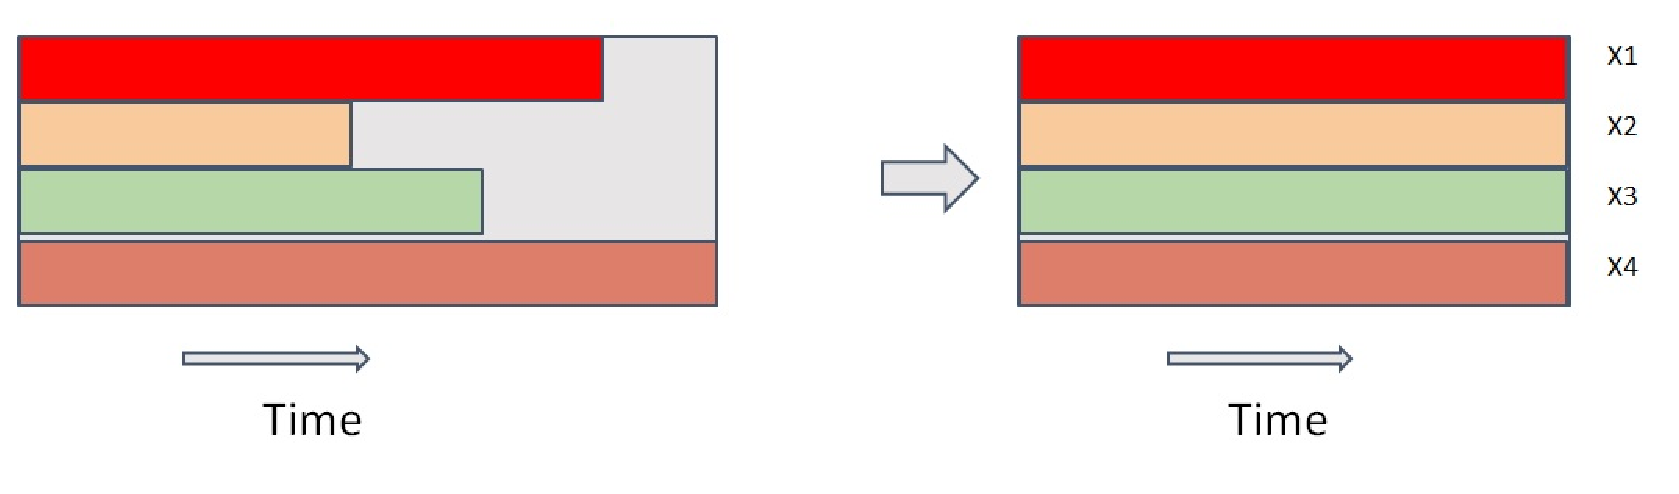
\includegraphics[scale=0.8]{Jacobi/EPS/time_diff.eps}
%}
%\caption{Expected Result of Power Aware Load Balancer}
%\label{fig:ideal}
%\end{figure}

    \begin{equation} \label{eq:3}
      (w_1x_1) = (w_2x_2) = (w_3x_3) = \dots = (w_nx_n) 
    \end{equation}
    \begin{equation} \label{eq:4}
      x_1 + x_2 + x_3 + \dots + x_n = N
    \end{equation}

  where, $w_i, 1 \leq i \leq n$ is the weight (in terms of times) for executing
  $x_i$ number of objects on processors PE$_i$ and $N$ is the total number of objects. 
  Before the load balancing all the x$_i$'s are the same as the Charm++
  runtime does an equal distribution of work on each processor. 
  The challenge is to choose the parameter $w_i$ in such a way that it correctly reflects the heterogeneity
  in performance of $i^{th}$ processor at lower power values and on the other hand  
  remain almost the same for higher power figures. We have chosen the metric of object time 
  for this purpose. The next subsection explains our  choice.
  %All the objects
  %have the same load/weight in terms of computation.  Each PE executes the same
  %number of objects before load balancing. Each PE before load balancing has
  %the same total load since each object has the same weight. 
  By using the above
  equation we get the proportionality based on which the number of objects need
  to be assigned while load balancing. For instance, processor PE$_1$ could
  be 2 times faster than PE$_2$ and P$_3$ could be 0.5 times faster than
  PE$_2$. In which case we will have the following proportionality: PE$_1$ :
  PE$_1$ : PE$_3$ = 2 : 1 : 0.5. Now based on this proportionality each processor is
  assigned such a load that everyone can finish their execution at the same
  point of time.  
  
  We use the both the equations (~\ref{eq:3}) and (~\ref{eq:4}) to determine
  $x_i$'s, $1 \leq i \leq n$, which is the new load for its respective
  processors that help finish all of them at almost the same time. The newly
  assigned load $x_i$ for each of the PEs is proportional to $w_i$ which we
  strive to reflect the relative speeds of the processors at a given power cap. 

\subsection{Selection of metric ``w''} 
We have considered processor idletime, processor background time
\footnote{Processor background time amounts to the overhead due to non
  migratable objects on that processor.} and processor object time \footnote{A
    processor's object time is defined as the sum of object times of all the
      objects executing on that processor.} as candidates for our selection.

      We measure these values for each processor at a power cap of 24W.
      Figures \ref{fig:idletime_bgtimevsproc} and \ref{fig:objtimevsproc} show
      the experimental plots.  The metric which has the maximum variance
      depicts the heterogeneity in the best possible way.  Percentage change
      between the maximum and minimum idle time was $0.35$, and the same for
      background time was $1.41$ and that of processor object time was $4.09$
      (This was partially due to a misbehavior of node0:core0 as seen in the
       Figure \ref{fig:objtimevsproc}).  Using the above observation we chose
      processor's object time as a metric for ``w'' because this shows the
      maximum variance at lower power caps. 
   

\begin{figure}
\begin{tabular}{cc}
  \scalebox{0.5}{
    \begin{tikzpicture}
  \begin{axis}[
   title = , 
   xlabel=  Core Ids,
   ylabel= Time (secs),
   ymax=2, ymin=0, xmax=60, xmin=0,
   x tick label style={black},
   grid=both
   ]
  \addplot table [x=PE, y=BG]{data2.dat};
  \addlegendentry {Overhead}
  \end{axis}
  \end{tikzpicture}
  }
& 
  \scalebox{0.5}{
    \begin{tikzpicture}
  \begin{axis}[
   title = , 
   xlabel=  Core Ids,
   ylabel= Time (secs),
   ymax=42, ymin=30, xmax=60, xmin=0,
   x tick label style={black},
   grid=both
   ]
  \addplot table [x=PE, y=I]{data2.dat};
  \addlegendentry {Idle Time}
  \end{axis}
  \end{tikzpicture}
  }
\\
\qquad (a) & \quad (b) \\
\end{tabular}
\caption{Idle and Overhead time over the cores at 24W power cap}
\label{fig:idletime_bgtimevsproc}
\end{figure}



\begin{figure}
\centering
  \scalebox{0.75}{
    \begin{tikzpicture}
    \begin{axis}[
     title = , 
     xlabel=  Core Ids,
     ylabel= Time (secs),
     ymax=58, ymin=11, xmax=60, xmin=0,
     x tick label style={black},
     grid=both
     ]
    \addplot table [x=PE, y=OBJ]{data2.dat};
    \addlegendentry {Collective Chare Time}
    \end{axis}
    \end{tikzpicture}
  }
\caption{{Processor object time on each processor at 24W power cap.}
\label{fig:objtimevsproc}
\end{figure}

%The idea  is drawn from the future guidelines of the work by Osman et
al.\cite{powerCluster2013} and \cite{osmanthesis}.  It has been empirically
observed that under the same power cap, different nodes yield different
application performance. This can be due to several design factors: difference
in chip designs, different in component assembly by the machine vendor,
   location of the node in the data center, difference in component design such
   as fans, etc. This difference in the design causes load imbalance across
   nodes despite same allocated power and equal compute load. Moreover we are
   going to experimentally show that this heterogeneity in nodes is more
   prominent at lower power caps.  Our goal is to minimize the load imbalance
   in the presence of such heterogeneity in nodes using the over-decomposition
   and dynamic object migration features of Charm++\cite{ChareKernelICPP90}. 

The rest of the presentation is organized as follows. Section~\ref{sec:approach}
depicts the detailed approach of our work. Section~\ref{sec:expr} gives the
experimental setup used and the results obtained. Finally the
Section~\ref{sec:fw} points out the conclusion and the future work.


\section{Results} \label{sec:results}
We used the existing Charm++ implementation of Jacobi2D and executed the
application at different power caps ranging from $23$ to $60 W$.  Each
execution of the Jacobi2D application (at a particular power cap) is done with
the following parameters:

\begin{enumerate}
\item Grid size                   = $ 36000 \times 36000$
\item Chare Size(or block size)   = $600 \times 600$
\item Number of Iterations        = $20$
\end{enumerate}

\subsection{Performance Evaluation Of Power Aware Load Balancer}
We run Charm++ applications (1) without load balancing (2) with existing load
balancing strategies (like  RefineLB and GreedyLB) and (3) with our Power Aware
strategy and the results are compared based on the the metrics of
heterogeneity, i.e. Equations \eqref{eq:1} and \eqref{eq:2}.  Power aware LB
has proved to be more efficient than other LBs. The main reason is the
frequency awareness our load balancer takes into account while trying to
minimize the load among the processors whereas RefineLB and GreedyLB are not aware of the
differences in frequency that exists at lower power caps. 
%This makes them power unaware. 
%They only consider the workload in terms of object wall time while
%balancing the load and try to converge to that point without taking into the
%account individual capacity of the processor. When migrating Chare objects from
%one node to other, our load balancer takes into account the existing
%workload and the time taken to complete the execution for that amount of
%workload, at both sending and receiving ends. This makes it perform well even
%in the presence of heterogeneity at lower power caps.

\begin{figure}
\centering
  \scalebox{0.75}{
    \begin{tikzpicture}
    \begin{axis}[
     xlabel=  Power Cap Values (W),
     ylabel = Total Execution Time (secs),
     ymax=34, ymin=5, xmax=60, xmin=23,
     x tick label style={black},
     grid=both
     ]
    \addplot table [x=POWER, y= PLB_MAX_TIME]{data.dat};
    \addlegendentry {Power Aware LB}
    \addplot table [x=POWER, y= WOLB_MAX_TIME]{data.dat};
    \addlegendentry {Without LB}
    \addplot table [x=POWER, y= RLB_MAX_TIME]{data.dat};
    \addlegendentry {Refine LB}
    \addplot table [x=POWER, y= GLB_MAX_TIME]{data.dat};
    \addlegendentry {Greedy LB}
    \end{axis}
    \end{tikzpicture}
  }
\caption{Total Execution Time Vs Power Comparison between LBs} 
\label{fig:final_exec_time_vs_power}
\end{figure}
%
As shown in Figure \ref{tb:1} a maximum speedup of 1.3$\times$ was seen when compared
to GreedyLB. Maximum speedup of 1.2$\times$ w.r.t to RefineLB and 1.28$\times$ w.r.t without LB.
The total execution time when run without any load balancer at 23W power cap is
~34sec.  This is somewhat reduced in case of RefineLB and GreedyLB. But the
power aware LB is able to decrease is to ~25sec as shown in figure
%\ref{fig:final_exec_time_vs_power}. The percentage decrease with the Power
Aware LB is more.

\begin{figure}[htbp]
  \begin{center}
  \scalebox{.75} {
     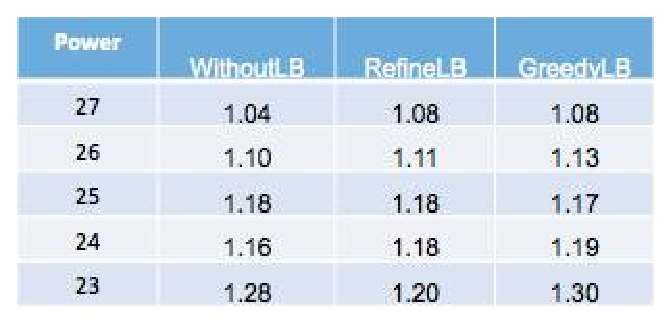
\includegraphics[scale=0.8]{Jacobi/EPS/t2.eps} 
  }
     \end{center}
  \caption{Speedups}
  \label{tb:1}
\end{figure}

There is little or no speed up in cases of higher power caps when using the
power aware load balancer. The reason behind this is the absence of
heterogeneity at higher power caps. The product of object wall time ‘w’ and the
workload ‘x’ comes to be almost the same, and so it leaves power aware LB no
scope of further balancing the workload based on frequency. Load imbalance is
observed only at lower power caps. Hence, there is very little migration that
power aware load balancer does at higher power caps. This makes GreedyLB
perform better at higher power caps, as it takes the greedy approach of freshly
loading the heaviest object with lightest loaded processor. 

GreedyLB and RefineLB are unaware of the differences in frequencies of
different nodes that exist at lower power caps. There is equal weightage given
to each node in GreedyLB and RefineLB. These do not take into account the
frequency of each node and assume that all the nodes in the cluster have
identical performance capability.


\begin{figure}
\centering
  \scalebox{0.75}{
    \begin{tikzpicture}
    \begin{axis}[
     xlabel=  Power Cap Values (W),
     ylabel = Average Idle Time (secs),
     ymax=15, ymin=0, xmax=60, xmin=23,
     x tick label style={black},
     grid=both
     ]
    \addplot table [x=POWER, y= PLB_AV_IDLE]{data.dat};
    \addlegendentry {Power Aware LB}
    \addplot table [x=POWER, y= WOLB_AV_IDLE]{data.dat};
    \addlegendentry {Without LB}
    \addplot table [x=POWER, y= RLB_AV_IDLE]{data.dat};
    \addlegendentry {Refine LB}
    \addplot table [x=POWER, y= GLB_AV_IDLE]{data.dat};
    \addlegendentry {Greedy LB}
    \end{axis}
    \end{tikzpicture}
  }
\caption{Average Idle Time vs Power Comparison between LBs}
\label{fig:avg_times_final_vs_power}
\end{figure}

\begin{figure}
\centering
  \scalebox{0.75}{
    \begin{tikzpicture}
    \begin{axis}[
     xlabel=  Power Cap Values (W),
     ylabel = Max Idle Time (secs),
     ymax=31, ymin=3, xmax=60, xmin=23,
     x tick label style={black},
     grid=both
     ]
    \addplot table [x=POWER, y= PLB_MAX_IDLE]{data.dat};
    \addlegendentry {Power Aware LB}
    \addplot table [x=POWER, y= WOLB_MAX_IDLE_P]{data.dat};
    \addlegendentry {Without LB}
    \addplot table [x=POWER, y= RLB_MAX_IDLE]{data.dat};
    \addlegendentry {Refine LB}
    \addplot table [x=POWER, y= GLB_MAX_IDLE]{data.dat};
    \addlegendentry {Greedy LB}
    \end{axis}
    \end{tikzpicture}
  }
\caption{Max Idle Time vs Power Comparison between LBs}
\label{fig:idle_times_final_vs_power}
\end{figure}


Performance of power aware LB is further analyzed with respect to other LBs in
terms of heterogeneity metrics – average idle time and max idle time, as shown
in Figure \ref{tb:2}. Power aware LB has out performed the other existing power
unaware LBs in terms of average and max idle times. The average idle time is
reduced using the power aware LB by as high as 60\% when compared to the
average idle time of the run without any LB. If compared with RefineLB and
GreedyLB, the reduction is as high as 54\% and 63\% respectively. The average
idle time at 23W comes to be ~12,10,14 and 5sec for runs without LB, with
Refine, Greedy and power aware LBs respectively as shown in figure
\ref{fig:avg_times_final_vs_power}.

\begin{figure}
  \begin{center}
  \scalebox{0.5} {
     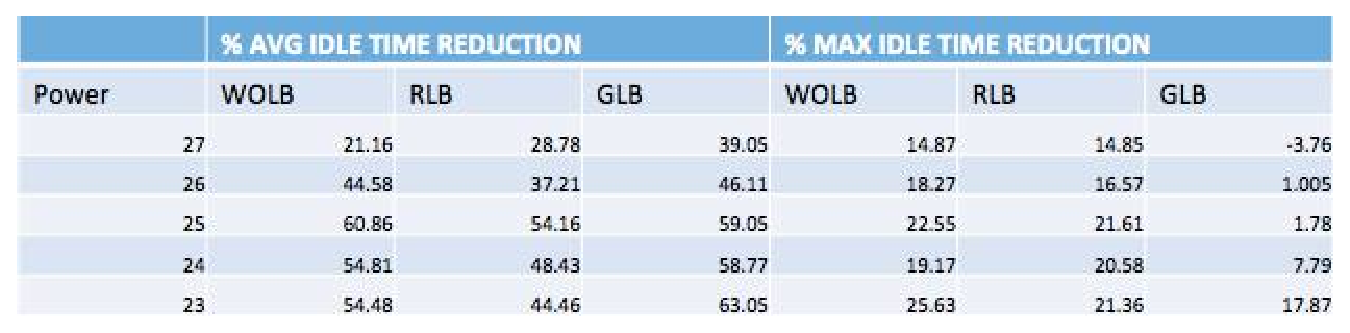
\includegraphics[scale=0.8]{Jacobi/EPS/t1.eps} 
  }
     \end{center}
  \caption{\% Reduction in Idle times}
  \label{tb:2}
\end{figure}

The reduction in maximum idle time is as high as 25\% in the presence of power
aware LB. It is ~30sec in the absence of any load balancer and it comes down to
~23sec when run with power aware LB at a low power cap of 23W as shown in
figure \ref{fig:idle_times_final_vs_power}. We could have further decreased
the maximum idle time. But due to an off node in the cluster with an unexpected
behavior led to an increased max idle time. However average idle time is a
better metric to measure the performance of our load balancer than the max idle
time since it’s taking average idle time into account and the misbehavior by a
one off node doesn’t pull the average down to a great extent unlike the max
idle time metric.

Power aware LB performs equally well in cases of higher power caps when there
is little or no heterogeneity among the nodes. One positive aspect here is that
power aware load balancer does not try to do unnecessary balancing at higher
power caps that could have led to an increase in the average or max idle
leading to an increase in the total execution time.

\begin{figure}
\centering
  \scalebox{0.75}{
    \begin{tikzpicture}
    \pgfplotsset{every axis legend/.append style={
          at={(0.5,1.03)},
          anchor=south}}
    \begin{axis}[
     xlabel=  Core Ids,
     ylabel= Total Execution Time (secs),
     ymax=34, ymin=2, xmax=60, xmin=0,
     x tick label style={black},
     grid=both
     ]
    \addplot table [x=PE, y= PLB]{data1.dat};
    \addlegendentry {With Power Aware LB}
    \addplot table [x=PE, y= RLB]{data1.dat};
    \addlegendentry {With Refine LB}
    \addplot table [x=PE, y= WOLB]{data1.dat};
    \addlegendentry {Without LB}
    \end{axis}
    \end{tikzpicture}
  }
\caption{Heterogeneity comparison between LBs at 23W} 
\label{fig:heter_final}
\end{figure}

Another observation of the total execution time is done on a per core basis at
23W. Figure\ref{fig:heter_final} depicts the amount of heterogeneity among the
nodes. Further from the same figure we can note that there is a lot of
difference in the total execution times by each node in the absence of any load
balancer. The total execution time ranges from 15-35 sec for the run without
any load balancer. RefineLB does not help in minimizing the heterogeneity by a
large extent. The range of total execution times remains close to 15-30 sec.
The power aware load balancer proves to redistribute the workload in a better
manner compared to existing Load Balancers.  As depicted in figure
\ref{fig:heter_final} the range of total execution time has decreased to 15-25
sec with most of the nodes closing to the average. The range could be further
reduced by making use of node specific information or hard coding based on
performance profiling of individual nodes. This profiling information is not
incorporated as they make the load balancer usable only for specific
applications running on known clusters.


\section{Conclusions \& Future Work} \label{sec:fw}
We observed that the execution time increases with decrease in CPU power, but
the rate at which it increases was seen to be different with some nodes
performing better than others, leading to performance heterogeneity. This leads
to some nodes exhibiting higher performance than others, and thus such nodes
tend to have higher idle-times waiting for other slower ones to complete their
iteration, before the next iteration could be started. Heterogeneity is
measured in terms of average idle times of the nodes in the cluster. This
heterogeneity becomes significant when the power is pulled down to the allowed
minimum. This load imbalance leads to more wait times among the nodes and thus
there is scope to minimize the imbalance by having a power aware load balancer
that gathers information of the initial few iterations and then based on the
collected information about the frequency and workload of different nodes,
          tries to bring down the idle times.  
 
To help mitigate this performance imbalance, we developed a power-aware load
balancer that helps in minimizing the heterogeneity. Our load balancer
performed better than the existing power-unaware load balancers in the Charm++
framework. It helped reduced the existing amount of heterogeneity and achieve a
maximum speed up of 1.3x with respect to other load balancers when used with
Jacobi2D application. 


The current limitation with this load balancer is that it does not take into
account the size of the workload on a particular node. This limits its usage in
the applications where the object size varies with time. One such applications
that we studied for heterogeneity at lower power regions was LeanMD\cite{leanmd}, where
there is particle migration happening as the application executes leading to
different object sizes at different times. 

Our future work aims at making our power-aware load balancer aware of the
changing size of the workload, and thus incorporating this parameter while
balancing the workload among the various nodes. This work also involves
periodic invocation of the load balancer in order to keep the idle times
minimized. This has to be done carefully, keeping the overall load balancing
workload to the minimum.



% use section* for acknowledgement
\section*{Acknowledgment}
We would like to thank Prof. Josep Torrellas for helping us procure the
resources required to establish the TestBed. The comments for the mid-term
review was very encouraging which motivated us further. We would also like to
thank Prof. Tarek Abdelzaher for giving us the permission for using the
physical machines which had the capability of power capping. This project would
not have been possible otherwise. We would like to thank the class of CS-533
itself for providing the opportunity to pursue this project. Finally, we would
like to thank Akhil and Osman, the PhD students of Prof. Laxmikant V. Kale, for
sharing their knowledge and inputs throughout the course of the project.

%\nocite{*}
\bibliographystyle{siam} \bibliography{bare_conf}
% that's all folks
\end{document}


